\documentclass{standalone}
\usepackage{tikz,xcolor}
\usetikzlibrary{calc}

% This code started as Jonthan Duncan't from Optima Statistics, but I ran it through AI to improve the colors, readability, and efficiency.
\begin{document}
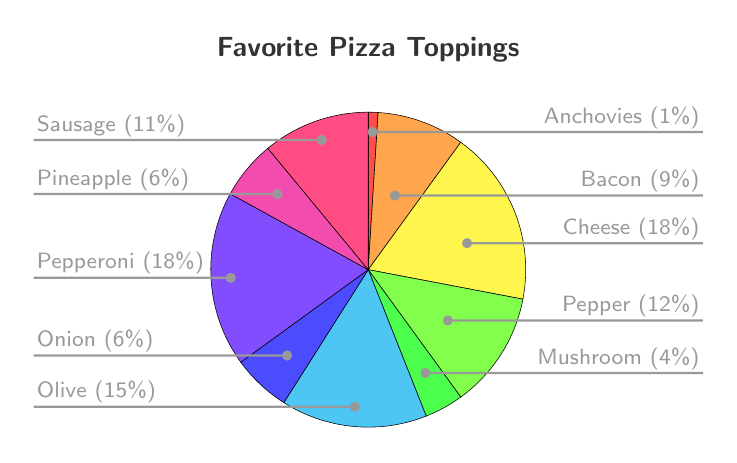
\begin{tikzpicture}

    % Calculate cumulative angles and draw pie slices
    \def\startangle{90}
    \def\currentangle{\startangle}

    % Loop through data to draw pie slices with bright colors
    \foreach \percentage/\label/\color [count=\i] in {
        1/Anchovies/red,
        9/Bacon/orange,
        18/Cheese/yellow,
        12/Pepper/green!70!yellow,
        4/Mushroom/green,
        15/Olive/cyan,
        6/Onion/blue,
        18/Pepperoni/blue!70!magenta,
        6/Pineapple/magenta,
        11/Sausage/red!70!magenta}
    {
        % Calculate end angle
        \pgfmathsetmacro{\endangle}{\currentangle - \percentage * 3.6}

        % Draw pie slice with bright colors
        \filldraw[fill=\color!70!white, draw=black, very thin]
            (0,0) -- (\currentangle:2) arc (\currentangle:\endangle:2) -- cycle;

        % Update current angle for next iteration
        \pgfmathsetmacro{\currentangle}{\endangle}
        \global\let\currentangle=\currentangle
    }

    % Establish precise coordinates for clean labeling (like first code)
    \coordinate (left border) at (4.25,0);
    \coordinate (right border) at (-4.25,0);
    \coordinate (l1) at (88.2:1.75);    % Anchovies
    \coordinate (l2) at (70.2:1.0);     % Bacon
    \coordinate (l3) at (15:1.3);       % Cheese
    \coordinate (l4) at (-32.5:1.2);    % Pepper
    \coordinate (l5) at (-61:1.5);      % Mushroom
    \coordinate (l6) at (-95.6:1.75);   % Olive
    \coordinate (l7) at (-133.4:1.5);   % Onion
    \coordinate (l8) at (-176.6:1.75);  % Pepperoni
    \coordinate (l9) at (-219.8:1.5);   % Pineapple
    \coordinate (l10) at (-250.3:1.75); % Sausage

    % Attach labels with clean positioning
    \begin{scope}[lab/.style={gray!80!white,thick,draw,font={\footnotesize\sffamily}},outer sep=-0.75mm]
      \fill[lab] (l1) circle(0.05) -- (l1-|left border) node[anchor=south east] {Anchovies (1\%)};
      \fill[lab] (l2) circle(0.05) -- (l2-|left border) node[anchor=south east] {Bacon (9\%)};
      \fill[lab] (l3) circle(0.05) -- (l3-|left border) node[anchor=south east] {Cheese (18\%)};
      \fill[lab] (l4) circle(0.05) -- (l4-|left border) node[anchor=south east] {Pepper (12\%)};
      \fill[lab] (l5) circle(0.05) -- (l5-|left border) node[anchor=south east] {Mushroom (4\%)};
      \fill[lab] (l6) circle(0.05) -- (l6-|right border) node[anchor=south west] {Olive (15\%)};
      \fill[lab] (l7) circle(0.05) -- (l7-|right border) node[anchor=south west] {Onion (6\%)};
      \fill[lab] (l8) circle(0.05) -- (l8-|right border) node[anchor=south west] {Pepperoni (18\%)};
      \fill[lab] (l9) circle(0.05) -- (l9-|right border) node[anchor=south west] {Pineapple (6\%)};
      \fill[lab] (l10) circle(0.05) -- (l10-|right border) node[anchor=south west] {Sausage (11\%)};
    \end{scope}

    % Enhanced title styling
    \node[font=\normalsize\sffamily\bfseries, color=black!80] at (0,2.8) {Favorite Pizza Toppings};

\end{tikzpicture}
\end{document}